\section{Three Chinese Encyclopedias}
The data sources for our association knowledge-base are Chinese Wikipedia,
Baidu Baike and Hudong Baike. Each article in three encyclopedias is
an unit for processing. The number of articles in Chinese Wikipedia,
Baidu Baike, Hudong Baike are 1 million, 7 million, and 4 million respectively.
All articles in data source are contributed by community
authors. Each article has a title which is a concept or an entity
and a body text which is used to describe the title.
%Figure \ref{figure:1} illustrates the
%structure of our data source.

%\begin{figure}[!h]
%    \centering
%    \subfigure[Data Source for Encyclopedia]{
%        \label{figure:1}
%        \includegraphics[width=5.5cm]{datasource.eps}
%    }
%    \hspace{0.5cm}
%    \subfigure[General Knowledge-Base Demonstration]{
%        \label{figure:2}
%        \includegraphics[width=5.5cm]{demo1_2.eps}
%    }
%    \caption{System Demo}
%\end{figure}
%
%The articles in three encyclopedias may have the same title.
%For example, three encyclopedias all have the article about Shanghai.
%But these three articles are different in the body text. We need to merge
%these three articles first. After merging, we got about 8 million
%articles which describe 8 millions entities.
%There are synonyms in our dataset. We linked the synonym to a synset.
%The synset has a representative title and a
%list of titles which are the synonyms of the representative title. Each synset has an article body to describe
%or explain this synset. Finally, we get 8 million synsets and each synset has an article to describe it.

The articles in three encyclopedias may have the same title.
For example, three encyclopedias all have the article about ``Shanghai.''
But these three articles are different in the body text. We first count those
two kinds of co-occurrence in each encyclopedia separately, and then merge
each kind of co-occurrence in three encyclopedias together. Then we get the merged
sentence-level co-occurrence and merged title-body co-occurrence.
Besides, there are synonyms in our dataset. We linked the synonym to a synset.
The synset has a representative title and a list of terms which are the synonyms of the representative title.
So we also merge co-occurrence related to words in the same synset together.
Finally, we get the merged sentence-level and title-body co-occurrence between synsets.
